\documentclass[tikz,border=8pt]{standalone}
\usepackage{xcolor}
\usetikzlibrary{arrows.meta,positioning}
\tikzset{
  head/.style={
    draw,
    rounded corners=4pt,
    minimum width=4.8cm,
    minimum height=0.95cm,
    text width=4.6cm,
    align=center,
    font=\small\bfseries,
    fill=gray!10
  },
  common/.style={
    draw,
    rounded corners=4pt,
    minimum width=4.0cm,
    minimum height=0.9cm,
    text width=3.8cm,
    align=center,
    font=\scriptsize,
    fill=blue!8
  },
  aave/.style={
    draw,
    rounded corners=4pt,
    minimum width=4.0cm,
    minimum height=0.9cm,
    text width=3.8cm,
    align=center,
    font=\scriptsize,
    fill=blue!10
  },
  bal/.style={
    draw,
    rounded corners=4pt,
    minimum width=4.0cm,
    minimum height=0.9cm,
    text width=3.8cm,
    align=center,
    font=\scriptsize,
    fill=green!9
  },
  uni/.style={
    draw,
    rounded corners=4pt,
    minimum width=4.0cm,
    minimum height=0.9cm,
    text width=3.8cm,
    align=center,
    font=\scriptsize,
    fill=orange!12
  },
  trace/.style={
    draw,
    rounded corners=4pt,
    minimum width=4.0cm,
    minimum height=0.9cm,
    text width=3.8cm,
    align=center,
    font=\scriptsize,
    fill=purple!10
  },
  flow/.style={->, >=Latex, thick, draw=gray!70}
}
\begin{document}
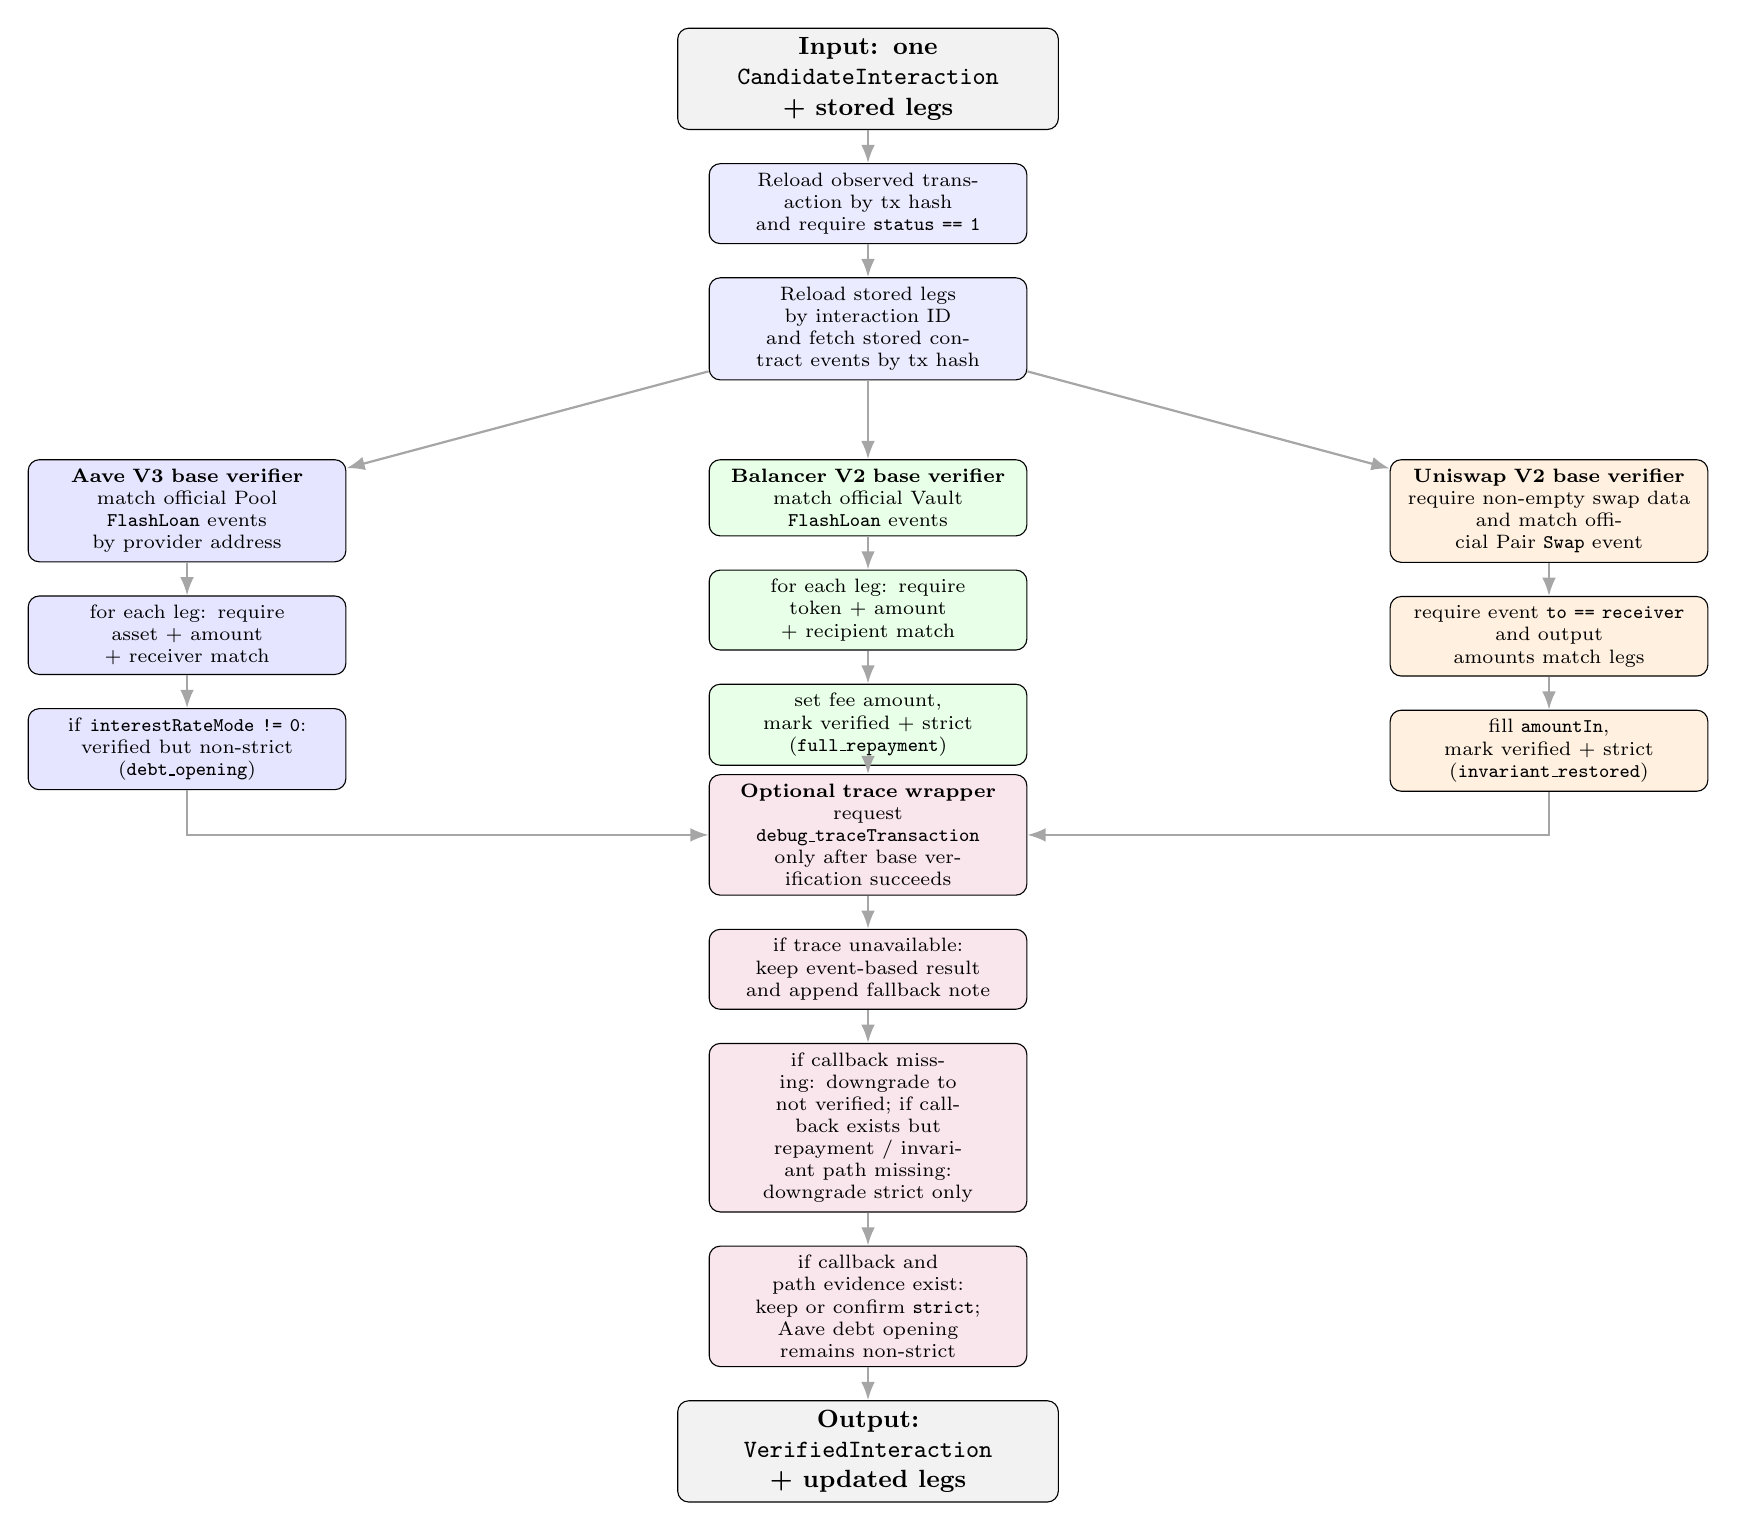
\begin{tikzpicture}[node distance=0.42cm]
  \node[head] (input) at (0,0) {Input: one \texttt{CandidateInteraction}\\+ stored legs};
  \node[common, below=of input] (common1) {Reload observed transaction by tx hash\\and require \texttt{status == 1}};
  \node[common, below=of common1] (common2) {Reload stored legs by interaction ID\\and fetch stored contract events by tx hash};

  \node[aave, below left=1.0cm and 4.6cm of common2] (a1) {\textbf{Aave V3 base verifier}\\match official Pool \texttt{FlashLoan} events\\by provider address};
  \node[aave, below=of a1] (a2) {for each leg: require\\asset + amount + receiver match};
  \node[aave, below=of a2] (a3) {if \texttt{interestRateMode != 0}:\\verified but non-strict\\(\texttt{debt\_opening})};

  \node[bal, below=1.0cm of common2] (b1) {\textbf{Balancer V2 base verifier}\\match official Vault \texttt{FlashLoan} events};
  \node[bal, below=of b1] (b2) {for each leg: require\\token + amount + recipient match};
  \node[bal, below=of b2] (b3) {set fee amount,\\mark verified + strict\\(\texttt{full\_repayment})};

  \node[uni, below right=1.0cm and 4.6cm of common2] (u1) {\textbf{Uniswap V2 base verifier}\\require non-empty swap data\\and match official Pair \texttt{Swap} event};
  \node[uni, below=of u1] (u2) {require event \texttt{to == receiver}\\and output amounts match legs};
  \node[uni, below=of u2] (u3) {fill \texttt{amountIn},\\mark verified + strict\\(\texttt{invariant\_restored})};

  \node[trace, below=5.0cm of common2] (t1) {\textbf{Optional trace wrapper}\\request \texttt{debug\_traceTransaction}\\only after base verification succeeds};
  \node[trace, below=of t1] (t2) {if trace unavailable: keep event-based result\\and append fallback note};
  \node[trace, below=of t2] (t3) {if callback missing: downgrade to\\not verified; if callback exists but\\repayment / invariant path missing:\\downgrade strict only};
  \node[trace, below=of t3] (t4) {if callback and path evidence exist:\\keep or confirm \texttt{strict};\\Aave debt opening remains non-strict};

  \node[head, below=of t4] (output) {Output: \texttt{VerifiedInteraction}\\+ updated legs};

  \draw[flow] (input) -- (common1);
  \draw[flow] (common1) -- (common2);

  \draw[flow] (common2) -- (a1);
  \draw[flow] (common2) -- (b1);
  \draw[flow] (common2) -- (u1);

  \draw[flow] (a1) -- (a2);
  \draw[flow] (a2) -- (a3);
  \draw[flow] (b1) -- (b2);
  \draw[flow] (b2) -- (b3);
  \draw[flow] (u1) -- (u2);
  \draw[flow] (u2) -- (u3);

  \draw[flow] (a3) |- (t1);
  \draw[flow] (b3) -- (t1);
  \draw[flow] (u3) |- (t1);

  \draw[flow] (t1) -- (t2);
  \draw[flow] (t2) -- (t3);
  \draw[flow] (t3) -- (t4);
  \draw[flow] (t4) -- (output);
\end{tikzpicture}
\end{document}
